\section{TULIP Academy}
%%==========================================================================================
%%
\begin{slide}{Director}
  \twocolumn[lcolwidth=0.7\linewidth,
rcolwidth=0.3\linewidth
]{
    \begin{itemize}
      \item Associate Professor Gang Li
      \begin{itemize}
        \item \textcolor{orange}{Deakin University}
          \begin{itemize}
            \item \textit{University Thesis Examination} Committee
            \item SEBE Faculty HDR Director
            \item Director for
                \begin{itemize}
                  \item \small{S578/S678/S778/S779 (Master of Information Technology)}
                \end{itemize}
            \item Founding Director for
                \begin{itemize}
                  \item \small{S306 (Bachelor of Computer Science)}
                  \item \small{S777 (Master of Data Science)}
                \end{itemize}
          \end{itemize}
        \item \textcolor{orange}{IEEE Technical Committee}
         \begin{itemize}
           \item Task Force on EDM (VC)
           \item Data Mining and Big Data Analytics (VC 2017)
           \item Enterprise Information Systems
           \item Enterprise Architecture and Engineering
         \end{itemize}
      \end{itemize}
    \end{itemize}}
    {\begin{flushleft}
       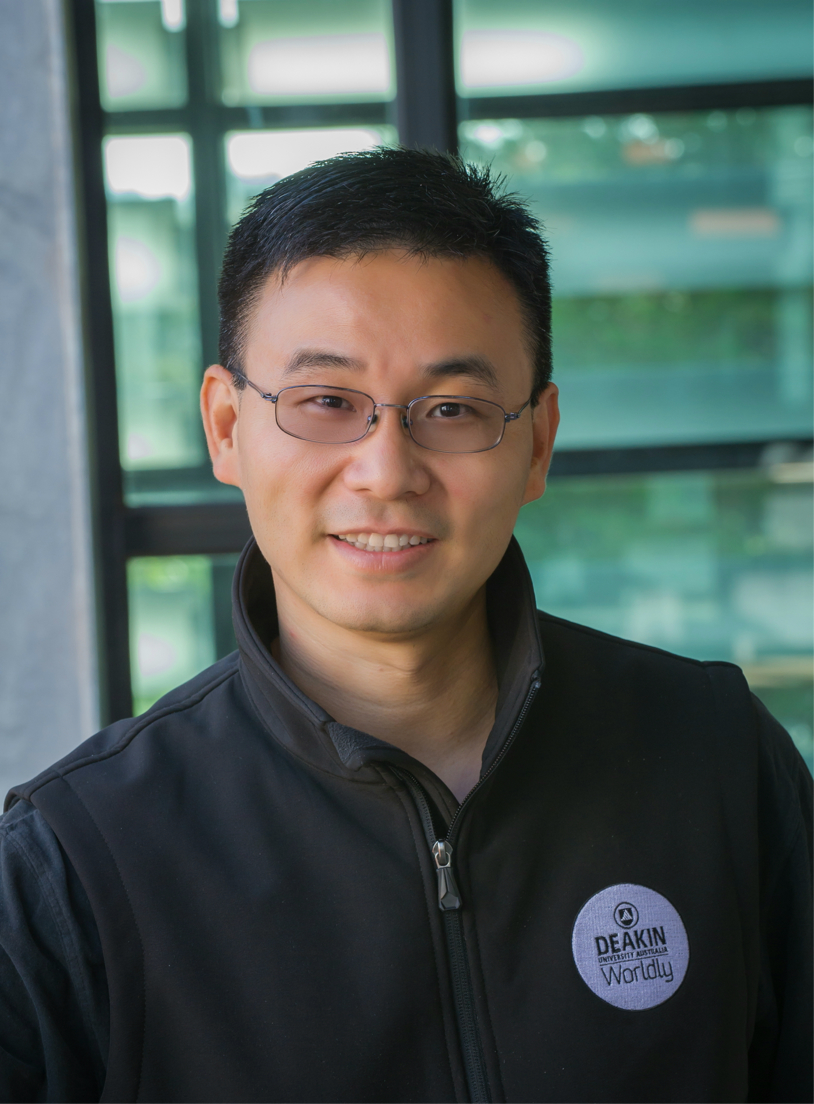
\includegraphics[width=0.8\textwidth]{figures//li//2014gangli.eps}
     \end{flushleft}
    }
\end{slide}
%%
%%===============================================================================


%%==========================================================================================
%%
\begin{slide}[toc=,bm=]{Deakin University}
	\begin{table}[htbp]
		\setlength{\abovecaptionskip}{-21pt}
		\setlength{\belowcaptionskip}{12pt}
		\centering
		\caption{Major Rankings of Deakin University}
		\begin{tabular}{l|c|cccc}
			\toprule
			& \textbf{Benchmark} & \multicolumn{1}{l}{\textbf{2014-2015}} & \multicolumn{1}{l}{\textbf{2015-2016}} & \multicolumn{1}{l}{\textbf{2016-2017}} & \multicolumn{1}{l}{\textbf{2017-2018}} \\ \midrule
			\multirow{2}[0]{*}{\textbf{ARWU}} & World & 301-400 & 201-300 & 201-300 & 201-300 \\
			& National  & 12-19 & 9-14  & 11-14  & 10-15 \\
			\midrule
			\multirow{2}[0]{*}{\textbf{CWTS Leiden}} & World  & 284 & 325 & 314 & 226 \\
			& National  & 11 & 17 & 17 & 11 \\
			\midrule
			\multirow{2}[0]{*}{\textbf{QS\#}} & World  & 360 & 324 & 355 & 293 \\
			& National & 19 & 17 & 19  & 17 \\
			\midrule
			\multirow{2}[0]{*}{\textbf{THE} } & World  & 301-350 & 301-350 & 251-300 & 301-350 \\
			& National  & 13-15 & 18-19  & 12-18  & 17-21 \\
			\midrule
			\multirow{2}[0]{*}{\textbf{THE<50}} & World  & 45 & 50 & 43  & 50 \\
			& National  & 6 & 8  & 8  & 8 \\
			\bottomrule
		\end{tabular}
		\label{tab:Deakin Ranking}
	\end{table}
	\centering
	\url{https://www.australianuniversities.com.au/rankings/}
\end{slide}
%%
%%==========================================================================================

%%==========================================================================================
%%

\begin{slide}{Organization}
\selectcolormodel{rgb}
\pgfkeys{/forest,
  rect/.append style   = { rounded corners = 2pt,
                         inner color = col6in, outer color = col6out},
  ellip/.append style  = { inner color = col5in,
                          outer color = col5out},
  orect/.append style  = { font = \sffamily\bfseries\LARGE,
                         text width = 325pt, text centered,
                         minimum height = 10pt, outer color = col7out,
                         inner color=col7in},
  oellip/.append style = { inner color = col8in, outer color = col8out,
                          font = \sffamily\bfseries\large, text centered}}
\begin{center}
\begin{forest}
  for tree={
      font=\sffamily\bfseries,
      line width=1pt,
      %draw=linecol,
      ellip,
      align=center,
      child anchor=north,
      parent anchor=south,
      drop shadow,
      l sep+=12.5pt,
      edge path={
        \noexpand\path[color=linecol, rounded corners=5pt,
          >={Stealth[length=11pt]}, line width=1pt, ->, \forestoption{edge}]
          (!u.parent anchor) -- +(0,-5pt) -|
          (.child anchor)\forestoption{edge label};
        },
      where level={3}{tier=tier3}{},
      where level={0}{l sep-=5pt}{},
      where level={1}{}{},
  }
    [TULIP Academy %inner color=col1in, outer color=col1out
    [Visitor]
    [Flipper
    [Trainee
        [[FLIP (00)]
          [\dots]
          [FLIP (05)]
        ]
    ]]
    [TULIP Lab
        [Australia]
        [China]
        [India]]
    [Alumni] %inner color =col7in, outer color = col7out]
    [Web Team] %, inner color=col2in, outer color=col2out]
  ]
\end{forest}
\end{center}
\end{slide}
%%
%%==========================================================================================


%%==========================================================================================
%%
\begin{slide}{Web Resources}
\begin{description}
\item[Official Websites]
  \begin{itemize}
    \item \textcolor{orange}{\faHome:} \url{http://www.tulip.org.au}
    \item \textcolor{orange}{\faGithub:} \url{https://github.com/tulip-lab}
  \end{itemize}

\item[Social Media]
  \begin{itemize}
    \item \textcolor{orange}{\faTwitter:} \href{https://twitter.com/tulipacademy}{tulipacademy}
    \item \textcolor{orange}{\faWeibo:} \href{https://weibo.com/tulipacademy}{tulipacademy}
    \item \textcolor{orange}{\faRedditAlien:} \url{https://www.reddit.com/r/tulipacademy}
  \end{itemize}

\item[Internal Services]
  \begin{itemize}
   \item \textcolor{orange}{\faBitbucket:} \url{https://bitbucket.org}
   \item \textcolor{orange}{\faCalendar:} \url{https://goo.gl/cWCWwC}
   \item \textcolor{orange}{\faCalendarCheckO:} \url{https://goo.gl/aC9VWW} (iCal)
  \end{itemize}

\end{description}
\end{slide}
%%
%%==========================================================================================
